\documentclass[tikz]{standalone}
\usepackage{chessboard}

\begin{document}
  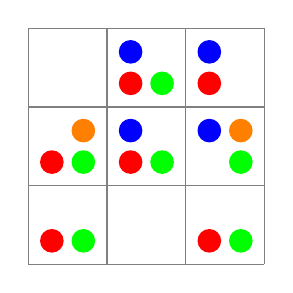
\begin{tikzpicture}
    \draw [gray] (0,0) grid (3, 3);
    \node at (0.5, 2.5) {\Huge \textcolor{red}{\symqueen}};
    \node at (1.5, 0.5) {\Huge \textcolor{black!20!green}{\symqueen}};
    \foreach \x/\y/\c in {
      0.3/0.3/red, 0.3/1.3/red, 1.3/1.3/red, 1.3/2.3/red, 2.3/0.3/red, 2.3/2.3/red,
      0.7/0.3/green, 0.7/1.3/green, 1.7/1.3/green, 1.7/2.3/green, 2.7/0.3/green, 2.7/1.3/green,
      1.3/1.7/blue, 1.3/2.7/blue, 2.3/1.7/blue, 2.3/2.7/blue,
      0.7/1.7/orange, 2.7/1.7/orange}
    {
      \fill[\c] (\x, \y) circle (0.15cm);
    }
  \end{tikzpicture}
  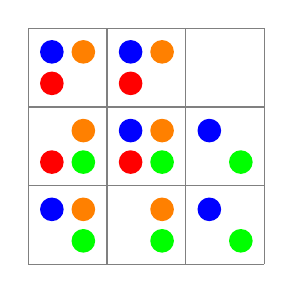
\begin{tikzpicture}
    \draw [gray] (0,0) grid (3, 3);
    \node at (2.5, 2.5) {\Huge \textcolor{blue}{\symqueen}};
    \foreach \x/\y/\c in {
      0.3/1.3/red, 0.3/2.3/red, 1.3/1.3/red, 1.3/2.3/red,
      0.7/0.3/green, 0.7/1.3/green, 1.7/0.3/green, 1.7/1.3/green, 2.7/0.3/green, 2.7/1.3/green,
      0.3/0.7/blue, 0.3/2.7/blue, 1.3/1.7/blue, 1.3/2.7/blue, 2.3/0.7/blue, 2.3/1.7/blue,
      0.7/0.7/orange, 0.7/1.7/orange, 0.7/2.7/orange, 1.7/0.7/orange, 1.7/1.7/orange, 1.7/2.7/orange}
    {
      \fill[\c] (\x, \y) circle (0.15cm);
    }
  \end{tikzpicture}
  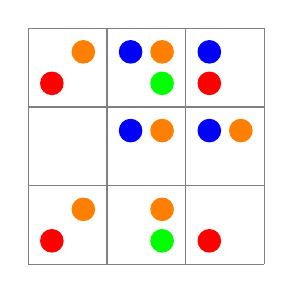
\begin{tikzpicture}
    \draw [gray] (0,0) grid (3, 3);
    \node at (0.5, 1.5) {\Huge \textcolor{orange}{\symqueen}};
    \foreach \x/\y/\c in {
      0.3/0.3/red, 0.3/2.3/red, 2.3/0.3/red, 2.3/2.3/red,
      1.7/0.3/green, 1.7/2.3/green,
      1.3/1.7/blue, 1.3/2.7/blue, 2.3/1.7/blue, 2.3/2.7/blue,
      0.7/0.7/orange, 0.7/2.7/orange, 1.7/0.7/orange, 1.7/1.7/orange, 1.7/2.7/orange, 2.7/1.7/orange}
    {
      \fill[\c] (\x, \y) circle (0.15cm);
    }
  \end{tikzpicture}
\end{document}
